\section{Privacy Enhancing Features}
Wownero is a privacy respecting memecoin\cite{wowbsite} and, as such, aims to provide users with strong anonymity and confidentiality. To achieve this, Wownero employs a range of privacy-enhancing features, including stealth addresses, ring signatures, RingCT, Dandelion+, and integration with TOR and I2P networks. The majority of these features were upstream inherited from Monero\cite{wowrepo,monero_repo}, but the Wownero developers have implemented some tweaks and modifications of their own.

% ------------------------------------------ %
\subsection{About Monero Addresses}
Conventional Bitcoin-like cryptocurrency addresses use a single key pair, similar to those used in \emph{RSA encryption}, but based on elliptic-curve cryptography\footnote{\textbf{Elliptic-curve cryptography} (ECC) uses the algebraic structure of elliptic curves over finite fields to perform cryptographic operations using smaller keys compared to conventional methods with the same level of security.}
\cite{zero2monero} rather than integer-factorization cryptography. Bitcoin wallet keys are generated using the ``Elliptic Curve Digital Signature Algorithm'' (ECDSA)\cite{ECDSA}. The key pair consists of a public key $(K)$ and a private key $(k)$ and, as is standard for asymmetric encryption, the public key is distributed freely (in the form of a derived address) while the private key must be carefully protected.

A standard Monero wallet address requires \emph{two} public-private key pairs. A view key $(K^v, k^v)$ and a spend key $(K^s, k^s)$\cite{monerodocs_addresses}. This double key pair system is a feature of CryptoNote coins and allows compartmentalization of access. For example, the view key can be shared to allow another party to audit incoming transactions and current balance without giving them the ability to send coins\cite{moneropedia}. Monero addresses are generated using the ``Edwards25519 Elliptic Curve'' signature scheme\cite{edwards_curve}.

I was curious what this curve looked like and plotted the positive and negative solutions to Curve25519 function in \texttt{Figure \ref{fig:curve}}. I do not believe this provides any greater understanding of the underlining mathematics, but now we know that it bears a striking visual similarity to a ``stick drawing'' of a fish.

\[y^2 = x^3+486662*x^2+x \implies \begin{cases}
y = +\sqrt{x^3 + 486662x^2 + x}\\
y = -\sqrt{x^3 + 486662x^2 + x}\end{cases}\]
\begin{figure}[H]
    \centering
    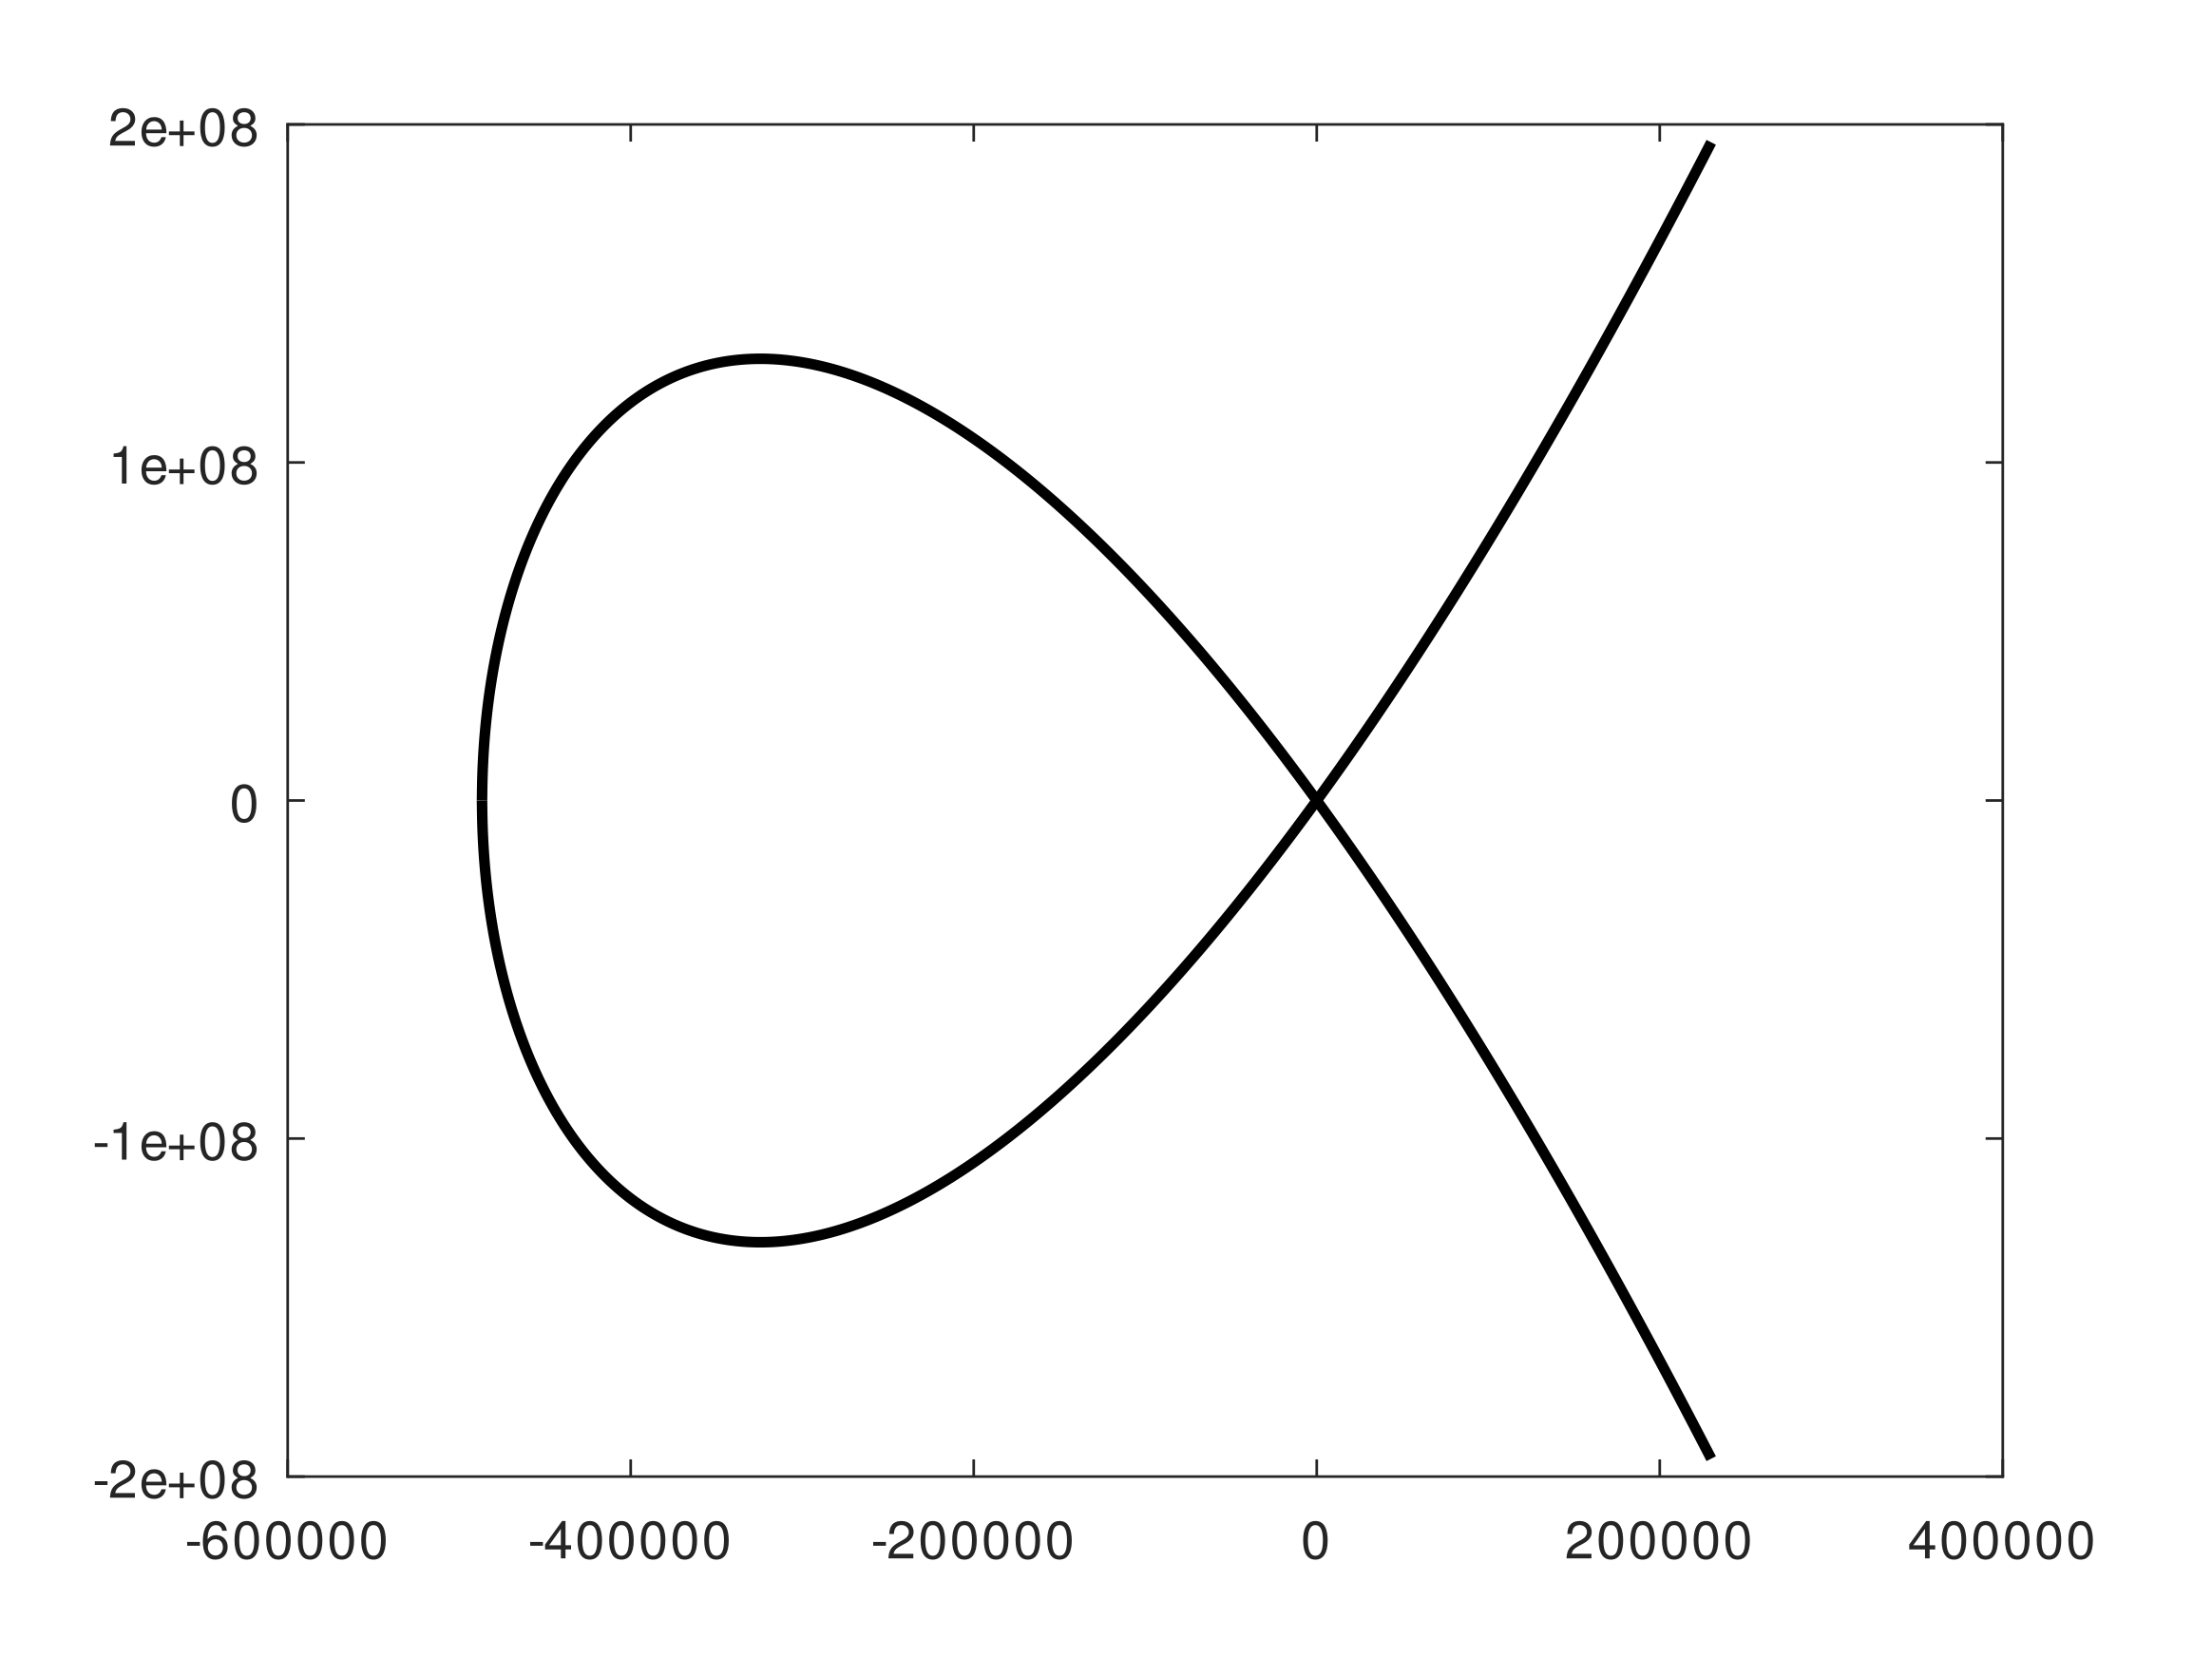
\includegraphics[width=300px]{curve}
    \caption{
        The Edwards25519 Elliptic Curve\\
        Image credit: \emph{\authorname}
    }
    \label{fig:curve}
\end{figure}

In addition to the public spend and view keys, Monero and Wownero addresses also contains a ``network byte,'' which makes the address network type identifiable, and a checksum to make mistyped addresses easily detectable\cite{monerodocs_addresses}. The complete anatomy of a Monero address is as follows:\cite{monerodocs_addresses} 
\begin{enumerate}
    \item A 1 byte network byte located at index 0.
    \item A 32 byte public spend key located at index 1.
    \item A 32 byte public view key located at index 33.
    \item The first 4 bytes of a hash of the rest of the key located at index 65.
\end{enumerate}

Most cryptocurrencies use base58 encoding, originally developed for Bitcoin\cite{zero2monero}, for the final address. Base58 is similar to base64 but omits the characters \texttt{I, O, l, 0, +, and /} to avoid ambiguity when read\cite{monerodocs_addresses}. Monero addresses use a modified version of base58 which performs the encoding in 8 byte blocks and pads the final block with $1$s\cite{monerodocs_addresses}. This produces a fixed size output ensuring all addresses are of the same length.

\medskip\noindent
An example final Monero address after base58 encoding into a 95 character string:\\
{\scriptsize\texttt{84DwgAEGE3NBeocw33eoj8ZjomhVYTQEuUKew8yvYJMxgfdDU9Y91BBgtvAX6dJ3PddVJRwe3trRcNku3fMEHc3A7XYmDbC}}\\
A main chain standard Monero address will always have an \emph{4} or \emph{8} as the first character\footnote{It is entirely coincidental that the example Monero address starts with 84}.

\medskip\noindent
An example final 97 character Wownero address:\\
{\scriptsize\texttt{WW33MLqvVUJZxDs4WkqgHn4SkTdKFn6hb2VAN8MBvENjfu2iug6p3CSJPDsVpggtEDZd715Xj4zy2jabweCV6WmY2kF6NMuZE}}\\

It appears that the reason for the longer address is due to the use of two bytes to represent the network. Because of this, every standard main chain Wownero address will start with \emph{Wo} or \emph{WW} at the cost of a pre-encoding address size of 70 bytes in length \emph{not} 69.

% ------------------------------------------ %
\subsection{Stealth Addresses}
``Stealth addresses,'' also known as ``one-time addresses,''\cite{zero2monero} allow the recipient address written to the blockchain to be a unique single-use address that cannot be linked to the original address \cite{stack_stealth}. Without stealth addresses it would be possible for an observer monitoring blockchain transactions to link transactions through heuristic pattern analysis of received transactions. For instance, linking a purchase of Monero via credit card to all other received payments would be trivial and completely de-anonymize the user.

The procedure for generating a stealth address was first described in the CryptoNote white paper\cite{CryptoNote} and has become one of the core Monero and Wownero privacy enhancing technologies\cite{moneropedia}.

\subsubsection{Stealth Address Cryptography} \label{sec:SA_example}
An example usage of a stealth address in a transaction between a sender, ``Shinji'', and a recipient, ``Rei'', will be explained\cite{zero2monero,CryptoNote,}. 

\noindent\textbf{[Sender] Shinji's Steps}
\begin{enumerate}
    \item Shinji initiates a Wownero transaction sending an amount, $a$, addressed to an address Rei provided.
    \item The wallet software separates the address into Rei's public view and send keys $(K^v_R, K^s_R)$
    \item A random number $r$ is selected ($r \in _R\mathbb{Z}_l$)\footnote{The $R$ indicates random selection from the set}\footnote{$l$ indicates exclusion of the Curve25519 infinity points from the set}.
    \item A one time address $K^o$ is calculated as 
    \[K^o=\mathcal{H}_s(rK^v_R, a)G+K^s_R\]
    \footnote{$G$ refers to the Ed25519 ``generator point'' on the curve which is the first point after infinity.}\footnote{$\mathcal{H}_s$ refers to a one-way cryptographic hash function.}
    \item The transaction is sent to the network with the one-time address $K^o$ as the recipient along with the value of $rG$.
\end{enumerate}
\noindent\textbf{[Receiver] Rei's Steps}
\begin{enumerate}
    \item Rei's wallet checks every transaction using her private view key. $k^v_R$ and
    \begin{enumerate}
        \item Multiplies her private view key $k^v_R$ by $rG$ ($rK^v_R = k^v_RrG$)
        \item Derives the original public send key $K'^s_R$ with 
        \[K'^s_R = K^o-\mathcal{H}_s(rK^v_R,a)G\]
        \item Transactions in which the derived send key match Rei's public send key ($K'^s_R=K^s_R$) are addressed to Rei.
    \end{enumerate}
    \item Having identified the transaction, the public and private spend keys for the output can be calculated.
    \begin{align*}
        K^o &= \mathcal{H}_s(rK^v_R,a)G+K^s_R\\
        &= (\mathcal{H}_s(rK^v_R,a)+k^s_R)G\\
        k^o &=\mathcal{H}_s(rK^v_R,a)+k^s_R
    \end{align*}
    Rei can now spend the received amount as desired using the spend key pair $(K^o, k^o)$ and the amount is added to his balance by the wallet software.
\end{enumerate}

Stealth addresses can be used optionally with non CryptoNote based coins, including Bitcoin, if both parties wallets support the feature\cite{stack_stealth}. Monero and Wownero \emph{require} their use and their respective wallets perform this automatically and transparently\cite{moneropedia}.

\subsubsection{View Tags}
As of the Monero v15 update on August 13, 2022\cite{monero_repo} and Wownero's very recent April 1st update codenamed ``Kunty Karen''\cite{wowrepo}, a new noteworthy piece of data was added to blocks. ``View Tags'' are 1-byte ``tags'' added to each transaction using a shared secret generated by the sender using the address provided to them by the recipient\cite{monero_viewtag}. Because all Monero transactions hide the recipient, wallet synchronization requires each transaction to be cryptographically decoded as described above to determine if the transaction is addressed to you.

The addition of view tags reduces sync times by $> 40\%$ by reducing the number of transactions which have to be fully checked (as shown in \ref{sec:SA_example} Receiver step 1) down to only 1/265th the total transactions\cite{monero_viewtag}.


\subsection{Subaddresses}
While Stealth Addresses protect you from 3rd parties linking transactions together, the \emph{sender} must necessarily know the address to which they are sending funds. ``Subaddresses'' allow a recipient to create a new publicly disclosable address for a transaction or category of transactions\cite{monerodoc_subaddr} allowing them to hide their primary address from even the person sending them funds\cite{moneropedia}.

The same functionality could be achieved by using multiple wallets, and for maximum unlinkability this remains the best option. Subaddresses exist to provide a convenience advantage over creating multiple wallets as they require a user to manage only a single seed phrase and keys\cite{monerodoc_subaddr}.

For an example of why this is necessary, suppose Rei utilizes the same address both to receive payments from an e-commerce business website and for personal use. Rei wins a bet and receives a personal payment from Shinji. By random chance Shinji is a customer of Rei's e-commerce site and recognizes the address revealing Rei as the operator of the site.

\subsubsection{Subaddress Cryptography}
To prevent this Rei creates a subaddress to receive the funds.
Both Monero and Wownero wallets make this very easy and the address is created as follows\cite{zero2monero}:
\begin{enumerate}
    \item Rei's public view and send keys are represented by $(K^v_R,K^s_R)$. The new $i$\textsuperscript{th}\footnote{$i$ represents the index of the subaddress. E.G. \{1,2,3\dots\}} subaddress keys will be represented by $(K^{v,i}_R,K^{s,i}_R)$
    \item Rei's subaddress is generated from his main address
    \begin{align*}
        K^{s,i} &= K^s:\mathcal{H}_s(k^v,i)G\\
        K^{v,i} &= k^vK^{s,i}
    \end{align*}
    So,
    \begin{align*}
        K^{v,i} &= K^v(k^s+\mathcal{H}_s(k^v,i))G\\
        K^{s,i} &= (k^s+\mathcal{H}_s(k^v,i))G
    \end{align*}\cite{zero2monero}
\end{enumerate}

The generated subaddress $(K^{v,1}_R,K^{s,1}_R)$ can then be used in transactions just like a primary address. As with a primary address, a stealth address will be generated from it, substituting $(K^{v,1}_R,K^{s,1}_R)$ for $(K^{v}_R,K^{s}_R)$ as
\[K^o=\mathcal{H}_s(rK^{v,1}_R, a)G+K^{s,1}_R\]

Rei's wallet will identify the received transaction, derive the transaction public send key (which will be the subaddress key $K^{s,1}_R$), and extract the one time keys for the transaction same as described in the \ref{sec:SA_example} transaction.

\subsubsection{Other Functionality}
Subaddresses are useful beyond privacy protection. For instance by providing a different subaddress for every expected payment it becomes easy to identify the purpose of a received payment\cite{monerodoc_subaddr}. For instance providing a different address to each of multiple tenants leasing a building would allow you to know who has paid their rent.
Subaddresses can also be used for more general categories rather than individual senders. For instance by categorizing into ``accounts'' for mining, work, personal, etc. or to wallet for separate business enterprises while retaining individual auditability\cite{monerodoc_subaddr}.


% ------------------------------------------ %
\subsection{Ring Signatures}
As stealth addresses and subaddresses ensure the anonymity of the recipient, ``ring signatures'' conceal the identity of the sender\cite{moneropedia}. Ring signatures, are a well established cryptographic Schnorr-like\cite{schnorr_sig} signing scheme\cite{ringsig_wikipedia}. They are special in that they allow any member of a group of users to cryptographically sign a message while protecting the identity of the individual signer\cite{ringsig_wikipedia}. They were developed by a group including Rivest and Shamir (well known for the \textbf{RS}A encryption scheme) and were first introduced at ASIACRYPT in 2001\cite{ringsig_wikipedia}. Ring signatures are a core part of any CryptoNote coins unlinkability guarantee, including Monero and Wownero\cite{CryptoNote,moneropedia,wowrepo}.

Ring signatures in Monero utilize a ``ring'' set of public keys, one of which must belong to the signer and the rest of which are used only as decoys. The primary feature of ring signatures over conventional ``group signatures'' is that it should be infeasible to determine which ring member was the actual signer\cite{zero2monero}. Under the CryptoNote protocol a random subset of other users public keys are used along with the transaction sender's key to form a ring\cite{CryptoNight}. 

For Wownero, the ring size is set to 22, which offers a \emph{theoretically} higher level of mixing compared to Monero which requires a ring size of 16\footnote{Monero formerly used a ring size of 11, but this was changed to 16 as part of the v15 update\cite{monero_repo}.}\cite{moneropedia}. This helps balance out Wownero's lower volume of transactions, users, and slower block time. While 16 or even 22 possible other addresses may not seem like a lot, this transaction mixing occurs for every transaction and over time the list of who may have transacted with any particular address will include almost everyone on the network\cite{monerohow_privacy}.

\subsubsection{Ring Signature Cryptography}
The procedure for signing and verifying a message $m$ with a ``Spontaneous Anonymous Group'' (SAG) ring signature $\mathcal{R}=\{K_1,K_2,\dots,K_n\}$ is as follows

\noindent\textbf{Transaction Signing}
\begin{enumerate}
    \item A random number $a$ is selected ($a \in _R\mathbb{Z}_l$).
    \item Multiple decoy responses $r$ of size $n=\text{ring size}-1$ are selected from a pool of addresses ($r_i \in \mathbb{Z}_l \text{ for } i \in \{1,2,\dots,n\}$)\footnote{$i$ refers to the index of the decoy response public key}.
    \item A challenge $c_{\pi+i}$ is calculated for the actual signer $i$ \footnote{$c$ is a created challenge which can only be proven using the private key.}\footnote{$\pi$ is an index referring to the actual signer's public key $K_\pi$ in the ring $\mathcal{R}$.}
        \[c_{\pi+1}=\mathcal{H}_n(\mathcal{R},m,[aG])\]
    \item Challenge values are calculated for each decoy response $i\in\{1,2,\dots,n\}$
        \[c_{i+1}=\mathcal{H}_n(\mathcal{R},m,[r_iG+c_iK_i])\]
    \item The real response value $r_\pi$ is defined such that $a=r_\pi+c_{\pi}k_{\pi}\pmod{l}$
    \item The signature $\sigma(m)$ is a tuple of the previously found values $\sigma(m)=(c_1,r_1,\dots,r_n)$
\end{enumerate}
The final complete ring signature consists of the signature $\sigma(m)$ and the full ring $\mathcal{R}$. \cite{zero2monero}


\noindent\textbf{Transaction Verification}
The signature $\sigma(m)$ can be proven by network nodes to correspond to a valid private key in ring $\mathcal{R}$
\begin{enumerate}
    \item We iterate over the set of ring entries $i\in\{1,2,\dots,n\}$ replacing $n+1 \rightarrow 1$ as \[c'_{i+1}=\mathcal{H}_n(\mathcal{R},m,[r_iG+c_iK_i])\]
    \item Any transaction in which the last term calculated is equivalent to $c_1$ is proven valid ($c_1=c'_1$). \cite{zero2monero}
\end{enumerate}

\subsubsection{Ring Signature Implementations}
Several variations of the described SAG ring signature have used for both Monero and Wownero in addition to the previously described SAG signature\cite{zero2monero}. At present time, both Monero and Wownero use Concise Linkable Spontaneous Anonymous Group (CLSAG) signatures as of October 2020\cite{moneropedia,wowrepo} which have provided a 10-25\% transaction size reduction\cite{moneropedia}. Here is a full list of signature schemes Monero has utilized \cite{zero2monero}
\begin{enumerate}
    \item Spontaneous Anonymous Group (SAG)
    \item Back's Linkable Spontaneous Anonymous Group (bLSAG)
    \item Multilayer Linkable Spontaneous Anonymous Group (ML-SAG)
    \item Concise Linkable Spontaneous Anonymous Group (CLSAG)
\end{enumerate}

% ------------------------------------------ %
\subsection{RingCT}
``RingCT'', or Ring Confidential Transactions\cite{ringct_whitepaper}, extends the ring signature protocol to also keep transaction \emph{amounts} private\cite{moneropedia}. Much as stealth addresses and ring signatures hide the identity of transaction participants, RingCT obfusicates the amount of funds sent\cite{moneropedia}. RingCT is build on Torben Pedersen's 1991 ``Pedersen commitment'' cryptographic scheme which is used to verify a secret's authenticity without disclosing any information about the secret\cite{penderson_commit_whitepaper}.

The feature was added to Monero in the January 2017 v4 update and has been required since September of the same year. Updates have since been made to the protocol such the 2018 v8 and 2022 v15 updates which implemented improvements to the ``Bulletproofs'' validation protocol\cite{monero_repo}. Wownero has utilized RingCT since launch with similar progressive updates upstreamed from Monero\cite{wowrepo}.

The signing process of a transaction using RingCT follows the steps outlined in the Ring Signature section with some additional steps for handling the transaction amounts. RingCT essentially creates a separate Penderson commitment for each member of the ring and only the holder of the recipients private key is able to discern the actual amount transfered\cite{ringct_whitepaper}. For RingCT, two ring signatures are combined using Schnorr signatures\cite{schnorr_sig} (later replaced by ``Borromean ring signatures''). One of these is necessary to prove the sum is 0 and the other is used to prove the outputs are positive numbers\cite{moneropedia}. To all external observers all transactions appear to be a commitment of 0 funds. Validation is done by confirming that all of the transaction's outputs are greater than zero using a range proof and proving that the sum of all outputs is zero (funds were neither created nor lost)\cite{ringct_whitepaper}.


\subsubsection{Bulletproofs}
The double ring signature scheme required for RingCT unfortunately resulted in a large transaction size and slow validation. This has been mitigated through the use of a new type of range proof called ``Bulletproofs''\cite{bulletproofs_whitepaper}. Bulletproofs are much more efficient type of range proof and validation of a large data set generates a comparatively  small proof which grows only logarithmically as the data size increases. Bulletproofs also have the ability to prove all transaction amounts at once without individual proofs of each output\cite{moneropedia}. 

Bulletproofs were added to Monero in the v8 update on October 18th 2018\cite{monero_repo} after a thorough audit process by three cryptography auditing organizations, \emph{QuarksLab} and  \emph{Kudelski Security} and a third which requested to be kept unnamed\cite{moneropedia}. Wownero's early Bulletproof implementation in the April 24th, 2018 ``Busty Brazzers'' update\cite{wowrepo} ahead of the full audit may have helped to validate the bulletproofs implementation before addition to Monero.

Since implementation of bulletproofs Monero's average transaction size has decreased by over 80\% which has been reflected in the transaction fees\cite{moneropedia}.

An improvement to the Bulletproofs protocol called ``Bulletproof+'' was later implemented to Monero as part of the September 13th, 2022 v15 update\cite{monero_repo}. Bulletproofs+ provide even more efficient range proofs for RingCT transactions with even smaller, faster to generate, and faster to verify proofs\cite{bulletproofs+}. This further reduces the transaction size and the computational burden on network nodes, making it possible for the blockchain to process more transactions without sacrificing security or privacy. For a ring size of 16, transactions are 10.8\% faster vs the original Bulletproofs\cite{bulletproofs+}. This upgrade was also integrated into Wownero ahead of Monero on July 4, 2021, in the ``Junkie Jeff'' update.


% ------------------------------------------ %
\subsection{Networking Privacy}
Monero and Wownero's commitment to privacy extends past the blockchain. Networking protocols are also utilized to hide which IP address was used to send a transaction and even hide the usage of the currency entirely. These protocols can be integrated into the blockchain node software or a separate user-configured optional addition.

\subsubsection{Dandelion++}
The nature of peer-to-peer node communication already makes discerning a transactions originating IP address quite difficult and would require an attacker to control a majority of nodes on the network\cite{localmonero-dandelion}. Dandelion++\cite{dandelion} is a privacy-enhancing feature which makes this already difficult attack virtually impossible even for a government level attacker. As the name implies, Dandelion++ is an upgraded version of the original 2017 Dandelion protocol which makes it more effective in cases in which many nodes disobey the protocol or do not use the Dandelion protocol at all\cite{dandelion}.


In an IP address identification attack carried out on network which uses conventional diffusion propagation \emph{without} Dandelion++ an attacker who controls many nodes on the network can monitor the order in which each node receives a transaction from one of their peers and deduce where the transaction originated based on the timing in which each node receives the transaction. If the attacker is able to successfully determine which node first encountered the transaction they can find the IP address which forwarded it to that node\cite{localmonero-dandelion}. By identifying the originating IP address, transactions can be linked despite features such as stealth addresses, subaddresses, or even entirely separate wallets. Against a state level attacker the IP address can be linked to the identity of the sender by the sender's internet service provider\cite{localmonero-dandelion}.

Dandelion++ mitigates this and obfuscates the diffusion order by propagating transactions in two phases determined by preset ``epoch'' intervals. Every epoch the node chooses whether to act as a ``Stem'' relay node or ``Fluff'' diffusion node until the next epoch, depending on a pseudo-random factor computed from a hash of the node identity and the epoch number\cite{dandelion}.

\begin{figure}[H]
    \centering
    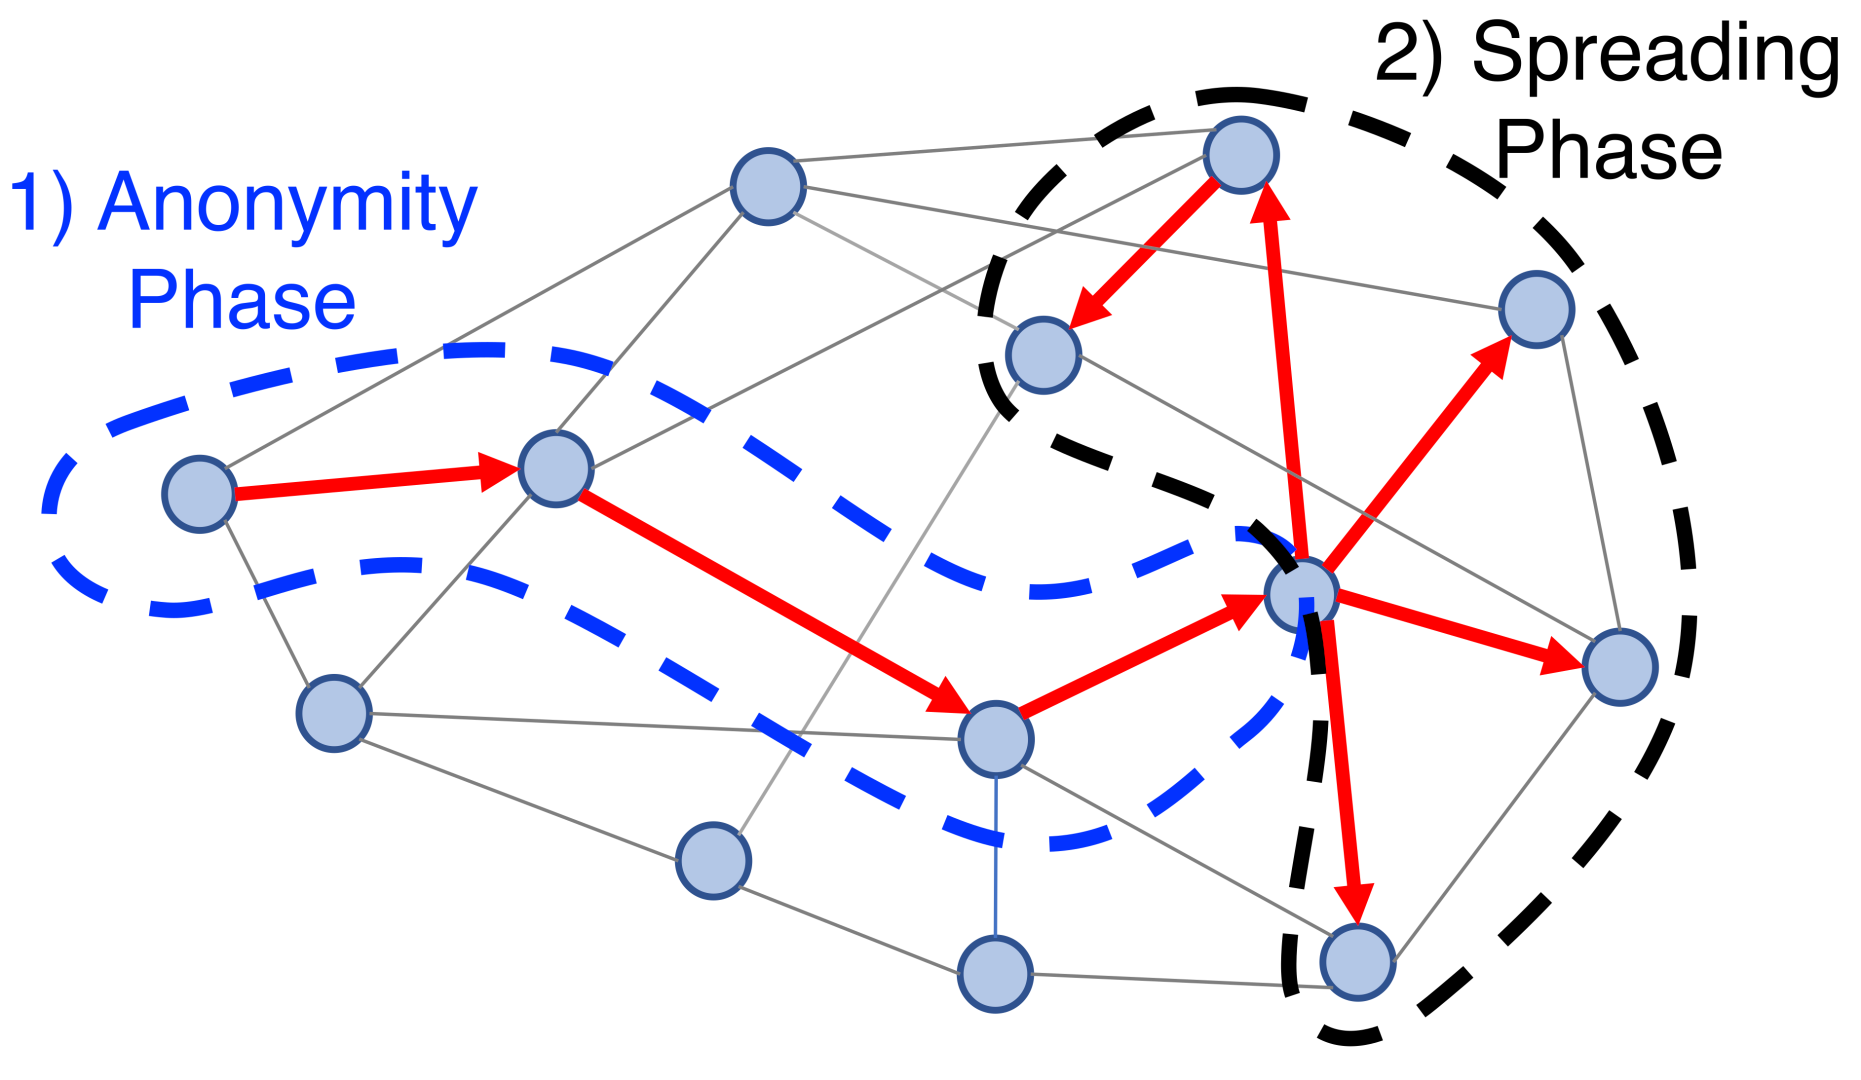
\includegraphics[height=160px]{dandelion}
    \caption{
        Phases of Dandelion Transaction Propagation\\
        Image source: ``Dandelion'' protocol white paper\cite{dandelion_original} 
    }
    \label{fig:dandelion}
\end{figure}

\noindent\textbf{``Stem'' Anonymity Phase}
In this phase, a 4-regular\footnote{a 4-regular graph is a graph in which every vertex is connected to exactly four other vertices.} anonymity graph of nodes are created (and re-generated every epoch)\cite{dandelion}. If the node is committing a new transaction of its own, it forwards the transaction along the same outbound edge in the anonymity graph\cite{localmonero-dandelion}.

Each time a node receives a stem-phase transaction from another node it relays transactions to two pseudorandomly chosen peers according to a map of incoming and outbound edges in the anonymity graph\cite{dandelion}.

\medskip
\noindent\textbf{``Fluff'' Spreading Phase}
In the spreading phase, the node propagates transactions over the network via the conventional diffusion method, transmitting the transaction to all of its connected nodes. This broadcasts the transaction to every outgoing connection with randomized communication times\cite{dandelion_original}.

\medskip
This two-stage method of propagation obfuscation makes an attacker unable to simply listen for the direction of a transaction. The stem phase nodes will have distributed the transaction randomly meaning the originating node of the fluff phase is not the source of the original transaction, and it is unknown how many hops along the stem the transaction underwent prior to mass propagation\cite{localmonero-dandelion}.


% ------------------------------------------ %
\subsection{Local vs Remote Nodes}
Because the Monero blockchain is quite large and can take a significant amount of time to sync (especially if using a mechanical hard drive) Monero wallets can connect to a ``Remote node'' rather than using a local node\cite{moneropedia}. Remote nodes, also known as public nodes, are not without potential drawbacks, however. A malicious remote node can easily see your IP address (negating the effectiveness of Dandelion+) and associate it with the transaction, hide blocks to make it appear as though your wallet is up-to-date, and provide a list of already spent decoy addresses reducing the effectiveness of ring signatures\cite{localmonero-remotenode}.

Despite the potential privacy compromises, using a remote node always remains secure as nodes are unable to manipulate transactions or access your private keys\cite{localmonero-remotenode}. Any concern of IP address transaction linking can be mitigated through the use of Tor, I2P, or a centralized VPN service such as ``Mullvad VPN.'' Remote nodes are sometimes the only option for wallets on mobile devices such as phones, Chromebooks, or laptops with insufficient free storage space. Using a remote node and conventional wallet is still preferable to using a ``light wallet'' such as ``MyMonero'' as these wallets handle all synchronization on an external server which requires access to your private view key, which gives complete access to inbound transaction history, in addition to all the potential risks of a remote node\cite{localmonero-remotenode}.

Monero wallets, like the internally developed desktop wallet ``Monero-Wallet-GUI,'' give the easy option of automatically configuring a local node or selection of a remote node. For Wownero there is very little need to use a remote node currently as, due to the lower transaction volume and more recent launch date, the blockchain database is much smaller..


\subsubsection{TOR}
``TOR,'' or ``The Onion Router,'' is a technology originally developed by the U.S. Navy which provides users with \emph{layers} of anonymity by routing traffic through many nodes and, theoretically, requiring an attacker to compromise all the nodes used to discern the original IP address of a user.
Monero can optionally be integrated with Tor and setup tutorials are provided in the Monero git repo documentation\cite{monero_repo}. The Monero and Wownero daemons provides a convenient command flag to connect to a Tor proxy running on localhost
\\\centerline{EX: \texttt{--tx-proxy tor,127.0.0.1:9050,10}}

\smallskip
Wownero's popular ``Wowlet''\cite{wowlet} wallet software uses Tor implicitly by default requiring no action on the part of the end user at all. 



\subsubsection{I2P}
``I2P,'' or the ``Invisible Internet Project,'' is another optional privacy protocol which can be used. There has been discussion and interest in future I2P integration with the Monero daemon, possibly through Kovri (discussed in section \ref{sec:kovri}), however this has been delayed\cite{kovri_repo}. I2P is intended to protect you from passive network monitoring, so that anyone observing network traffic cannot tell that Monero is being used at all. The Monero developers prefer I2P over TOR because of its more decentralized routing protocol and asymmetric connections which mitigate 'timing attacks'\cite{monerohow_privacy}. Currently, the Wownero endorsed I2P router is i2p-zero\cite{i2pzero_repo}. As with Tor a command line flag is available to connect to an I2P proxy running on localhost
\\\centerline{EX: \texttt{--tx-proxy i2p,127.0.0.1:90000}}

\subsubsection{Kovri} \label{sec:kovri}
Kovri is a privacy-focused network layer that based on the I2P specification developed by the Monero Research Lab\cite{kovri_repo}. Kovri is not (yet) part of Monero however it may be added in a future update after a thorough evaluation and security audit\cite{moneropedia}. Because of Wownero's historically less stringent testing requirements Kovri could be implemented into Wownero ahead of Monero.

Kovri aims to be an easy to use, maintain, and review I2P router with extended functionality such as a ``hidden mode'' which would make I2P usage harder to detect by an internet service provider\cite{kovri_repo}. That feature could help to make Monero and Wownero more available in totalitarian countries with a highly controlled internet. Kovri is a rewrite of I2P in C++, forked from the i2pd project, for higher performance and to remove dependence on a bulky Java runtime\cite{kovri_repo}.

Their seems to be some hostility between I2P and Kovri developers as shown in the Kovri FAQ section ``Why did you fork from i2pd?'' \cite{kovri_repo}
\begin{quote}
    \dots We wanted a positive community that encouraged collaboration for the betterment of the software; not negative, narcissist glory\dots [and] a lead developer who could lead; not someone who could ignore requests for responsible disclosure or tuck-tail-and-run when faced with collaborator conflict
\end{quote}
Hopefully this disagreement will not jeopardize future development of either of these privacy-enhancing projects, however, the Kovri project may have been abandoned already as the last commit was 3 years ago and public enthusiasm towards the project has declined. 


